\newif\ifglobal

%%%%%%%%%%%%%%%%%%%%%%%
%%% Compile to view %%%
%%%%%%%%%%%%%%%%%%%%%%%

%%%%%%%%%%%%%%%%%%%%%%%%%%%%%%%%%%%%%%%%%%%%%%%%%%%
%%% Readme:                                     %%%
%%% https://www.overleaf.com/read/bwdjvfjksvjy/ %%%
%%%%%%%%%%%%%%%%%%%%%%%%%%%%%%%%%%%%%%%%%%%%%%%%%%%

% >>> M?: marks a module setting number or important notice

% >>> M4: Set {./relative-path} to external files for this module <<<
\def \modulefiles {./28-LEDPWM}
% To add an external file, use:
% (Replace '---' with actual filename)
% '\input{\modulefiles/tables/---.tex}' for tables
% '\includegraphics{\modulefiles/figures/---}' for figures
% '\subfile{\modulefiles/---}' for register files


% >>> M1: This module is in global project? <<<
% 'YES' - uncomment; 'NO' - comment out
\globaltrue

\ifglobal
    \documentclass[main\_\_CN.tex]{subfiles}

\else
    % Font "FandolSong-Regular" used by ctex does not have GSUB table.
    % It causes warnings that do not affect compilation and can be ignored.
    \PassOptionsToPackage{quiet}{fontspec}

    \documentclass[openany, 10pt]{book}

    % >>> M2: In ./00-shared/preamble-trm-module, also find
    %         settings for visibility of todo notes, watermark <<<
    \usepackage{preamble-trm-module}

    % Enable Chinese typesetting
    \usepackage{ctex}

    % >>> M3: Temporary labels in Chinese
    %         you can add your own labels there <<<
    \myexternaldocument{./00-shared/temp-labels-cn}

\fi %\ifglobal


\setcounter{secnumdepth}{4}


% >>> M5: If this module needs any updates in
% './00-shared/preamble-trm-module.sty'
% (include additional package, etc.), contact your module PM
% or create the file './00-shared/changelog.tex' make the
% necessary updates yourself and document them in this file <<<

% Make text left-aligned and allow latex to break pages naturally, comment out for full justification
\raggedright
\raggedbottom


\begin{document}


% Sets language into which pre-defined bits of text are translated
\selectlanguage{chinese}
\setchineseformatting


% Do not delete this block
\ifglobal
% Add the following front matter if
% this module is outside of global project
\else
    \InputIfFileExists{readme}{}{}
    \listoftodos
    {\let\clearpage\relax \listofdonetodos}
    \tableofcontents
    %\listoftables
    %\listoffigures
\fi


%%%%%%%%%%%%%%%%%%%%%%%%%
%%% TRM Module Begins %%%
%%%%%%%%%%%%%%%%%%%%%%%%%

\hypertarget{ledpwm}{}
\chapter{LED PWM 控制器 (LEDC)}
\label{mod:ledpwm}
\section{概述}

LED\_PWM 主要用于控制 LED 的亮度和颜色，也可以产生 PWM 信号用于其他用途。LED\_PWM 有 16 路通道，即 8 路高速通道和 8 路低速通道。这 16 路通道能够产生独立的数字波形来驱动 RGB LED 设备。 高速或低速通道可以由四个高速定时器之一或四个低速定时器之一进行驱动。PWM 控制器还能够自动逐渐增加或减少占空比，在无须处理器干预的情况下实现亮度和颜色渐变。LED\_PWM 还支持小数分频。

在本文中，hsch\textcolor{red}{\it{n}} 指高速通道，lsch\textcolor{red}{\it{n}} 指低速通道。高速定时器和低速定时器分别命名为 h\_timer\textcolor{red}{\it{x}} 和 l\_timer\textcolor{red}{\it{x}}。

\section{功能描述}

\subsection{架构}
图 \ref{Figure:led_pwm_architecture} 为 LED\_PWM 基本架构图。从图中可知，LED\_PWM 内部有 8 个高速通道以及 8 个低速通道。高速通道有 4 个高速时钟模块，可以从中任选一个 h\_timer\textcolor{red}{\it{x}}。低速通道有 4 个低速时钟模块，可以从中任选一个 l\_timer\textcolor{red}{\it{x}}。

\begin{figure}[H]
    \centering
    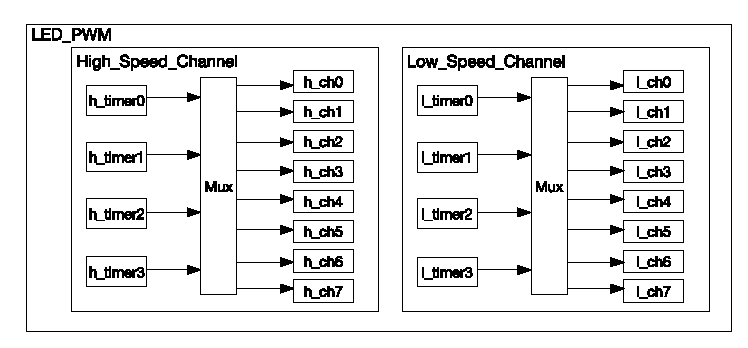
\includegraphics[width=0.7\textwidth]{./28-LEDPWM/figures/led_pwm_architecture}
    \caption{LED\_PWM 架构}
    \label{Figure:led_pwm_architecture}
\end{figure}

图 \ref{Figure:led_pwm_high_speed_channel} 表示一个 PWM 通道和它选取的分频器； 在该情况下，一个高速通道配有一个高速分频器。

\begin{figure}[H]
    \centering
    
\includegraphics[width=0.7\textwidth]{./28-LEDPWM/figures/led_pwm_high_speed_channel}
    \caption{LED\_PWM 高速通道框图}
    \label{Figure:led_pwm_high_speed_channel}
\end{figure}
\newpage
\subsection{分频器}\label{ledc_timers}

\begin{figure}[H]
    \centering
    \fbox{
\includegraphics[width=0.9\textwidth]{./28-LEDPWM/figures/ledc_frag_div}}
    \caption{LED\_PWM 分频器}
    \label{Figure:led_pwm_divider}
\end{figure}

LED PWM 高速定时器的时钟 LEDC\_CLK\regindex{x} 有两个时钟源：REF\_TICK 和 APB\_CLK（关于时钟源的更多信息请参考章节\hyperref[mod:resclk]{复位和时钟}）。输入时钟首先由分频器进行分频，分频系数为 LEDC\_CLK\_DIV\_NUM\_HSTIMER\textcolor{red}{\it{x}}，该系数的固定位宽是 18 位：其中高 10 位为整数部分 A，低 8 位为小数部分 B。分频系数 LEDC\_CLK\_DIV\regindex{x} 的公式为：
\begin{center}
$LEDC\_CLK\_DIV\regindex{x} =A + \frac{B}{256}$
\end{center}
分频系数的范围为 1 $\sim$ 1023。

小数部分不为 0 时，分频器的输入输出时钟如图 \ref{Figure:led_pwm_divider} 所示。256 个输出周期中有 B 个周期以 (A+1) 分频，有 (256-B) 个周期以 A 分频。以 (A+1) 分频的 B 个周期均匀分布在 256 个周期中。

分频器的输出时钟作为计数器的基准时钟，计数器的计数范围由 LEDC\_HSTIMER\textcolor{red}{\it{x}}\_DUTY\_RES 进行配置，每次计数达到最大值 $2^{LEDC\_HSTIMER\textcolor{red}{x}\_DUTY\_RES}-1$ 时，产生溢出中断， 并且计数值回归到 0。软件可以复位、 暂停以及读取计数器的计数值。

定时器的输出信号由计数器产生，位宽为 20 位。信号的循环周期决定了任何连接到该定时器的 PWM 通道的信号频率。

PWM 生成器输出信号 sig\_out\regindex{n} 的频率取决于定时器时钟源 LEDC\_CLK\regindex{x} 的频率、 时钟分频系数 LEDC\_CLK\_DIV\regindex{x} 以及占空比精度（计数器位宽）LEDC\_HSTIMER\regindex{x}\_DUTY\_RES：

    \[
    f_{\textrm{sig\_out\regindex{n}}}=\frac{f_{\textrm{LEDC\_CLK\regindex{x}}}}
                        {\textrm{LEDC\_CLK\_DIV}\regindex{x}\cdot 2^{\textrm{LEDC\_HSTIMER}\regindex{x}\_\textrm{DUTY\_RES}}}
    \]

上述公式变形后，可得到以下公式计算预期的占空比精度：

    \[
    \textrm{LEDC\_HSTIMER\regindex{x}\_DUTY\_RES}
    =\log_2\left(\frac{f_{\textrm{LEDC\_CLK\regindex{x}}}}
    {f_{\textrm{sig\_out\regindex{n}}}\cdot \textrm{LEDC\_CLK\_DIV\regindex{x}}}\right)
    \]

表 \ref{tab:ledc-common-freq-res} 列出了常用配置频率及其对应精度。

\begin{ThreePartTable}

    \begin{TableNotes}

        \item[1] 最高精度指时钟分频系数 LEDC\_CLK\_DIV\regindex{x} 为 1 时的精度，向下取整。如果经公式计算出的最高精度超过了计数器位宽 20 位，则最高精度为 20。

        \item[2] 最低精度指时钟分频系数 LEDC\_CLK\_DIV\regindex{x} 为 $1023+\frac{255}{256}$ 时的精度，向上取整。如果经公式计算出的最低精度小于 0，则最低精度为 1。

    \end{TableNotes}

\begin{longtable}[c]{ | l | l | l | l | }
\caption{常用配置频率及精度}
\label{tab:ledc-common-freq-res}
\\\hline
\rowcolor{lightgray}
LEDC\_CLK\regindex{x} & PWM 频率 & 最高精度（位） \tnote{1} & 最低精度（位）\tnote{2} \\\hline

\endhead
\insertTableNotes
\endfoot

APB\_CLK (80 MHz) & 1 kHz & 16 & 7 \\\hline
APB\_CLK (80 MHz) & 5 kHz & 13 & 4 \\\hline
APB\_CLK (80 MHz) & 10 kHz & 12 & 3 \\\hline
RC\_FAST\_CLK (8 MHz) & 1 kHz & 12 & 3 \\\hline
RC\_FAST\_CLK (8 MHz) & 2 kHz & 11 & 2 \\\hline
REF\_TICK (1 MHz) & 1 kHz & 9 & 1 \\\hline
\end{longtable}
\end{ThreePartTable}





低速通道的分频器 l\_timer\textcolor{red}{\it{x}} 相对于高速通道的分频器 h\_timer\textcolor{red}{\it{x}} 来说有以下 2 点区别：

\begin{enumerate}
    \item 高速定位器的时钟源采用了 REF\_TICK 或  APB\_CLK，低速定位器采用了 REF\_TICK 或 SLOW\_CLOCK。置位 LEDC\_APB\_CLK\_SEL 寄存器，SLOW\_CLOCK 的频率为 80 MHz，否则为 8 MHz。
    \item 当软件修改了高速通道计数器的最大值或分频系数的话，输出信号的更新将会在下一次溢出中断之后生效。而低速通道在置位 LEDC\_LSTIMER\textcolor{red}{\it{x}}\_PARA\_UP 之后，立刻更新计数器的计数范围参数和分频器的分频系数。
\end{enumerate}

\subsection{通道}\label{LEDCchannel}

每个通道有两个比较器，即图 \ref{Figure:led_pwm_high_speed_channel} 中的 high\_level\_comparator 以及 low\_level\_comparator。high\_level\_comparator 的比较值是 hpoint，由 LEDC\_HPOINT\_HSCH\textcolor{red}{\it{n}} 配置。当计数器的值达到 hpoint 时，输出信号翻转为高电平。\\
low\_level\_comparator 的比较值是 lpoint，由 LEDC\_DUTY\_HSCH\textcolor{red}{\it{n}}， LEDC\_DUTY\_START\_HSCH\textcolor{red}{\it{n}}， \\ LEDC\_DUTY\_INC\_HSCH\textcolor{red}{\it{n}}， LEDC\_DUTY\_NUM\_HSCH\textcolor{red}{\it{n}} 以及 LEDC\_DUTY\_SCALE\_HSCH\textcolor{red}{\it{n}} 共同决定。当计数器的值等于 lpoint 时，输出信号翻转为低电平。图 \ref{Figure:led_pwm_fixed_duty} 为 LED\_PWM 输出信号图。

\begin{figure}[H]
    \centering
    \fbox{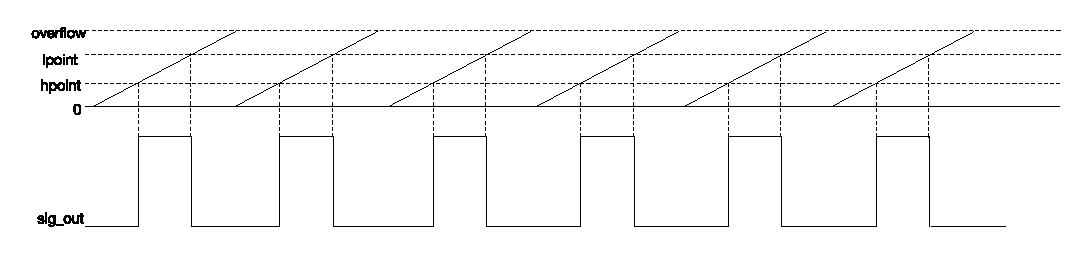
\includegraphics[width=0.7\textwidth]{./28-LEDPWM/figures/led_pwm_fixed_duty}}
    \caption{LED\_PWM 输出信号图}
    \label{Figure:led_pwm_fixed_duty}
\end{figure}


\label{ledcfd:dithering}
LEDC\_DUTY\_HSCH\textcolor{red}{\it{n}} 是一个具有 4 位小数的浮点寄存器，其中高 20 位是整数部分，低 4 位是小数部分。当低 4 位非 0 时，输出信号的脉冲宽度有 LEDC\_DUTY\_HSCH\textcolor{red}{\it{n}}［3：0]/16 的概率多一个计数周期。低 4 位小数有利于提高输出信号占空比的精度。置位 LEDC\_DUTY\_START\_HSCH\textcolor{red}{\it{n}}，通道更新后的 LEDC\_DUTY\_HSCH\textcolor{red}{\it{n}} 寄存器值才会起作用，即通道可以实现一种占空比到另一种占空比的转换。

LEDC\_DUTY\_INC\_HSCH\textcolor{red}{\it{n}} 决定了占空比的变化方向。渐变占空比的定义如下：\\
每 LEDC\_DUTY\_CYCLE\_HSCH\textcolor{red}{\it{n}} 个脉冲， LEDC\_DUTY\_HSCH\textcolor{red}{\it{n}}的高 20 位就会递增或递减\\ LEDC\_DUTY\_SCALE\_HSCH\textcolor{red}{\it{n}}，渐变长度由 LEDC\_DUTY\_NUM\_HSCH\textcolor{red}{\it{n}} 控制，当渐变完成后，会产生渐变完成中断，且之后的输出信号将延续最后一次脉冲。图 \ref{Figure:led_pwm_unfixed_duty} 为 LEDC\_DUTY\_INC\_HSCH\textcolor{red}{\it{n}} 为 1 时的渐变图，即每隔 LEDC\_DUTY\_CYCLE\_HSCH\textcolor{red}{\it{n}} 个脉冲，输出信号脉宽递增 LEDC\_DUTY\_SCALE\_HSCH\textcolor{red}{\it{n}}。

\begin{figure}[H]
    \centering
    \fbox{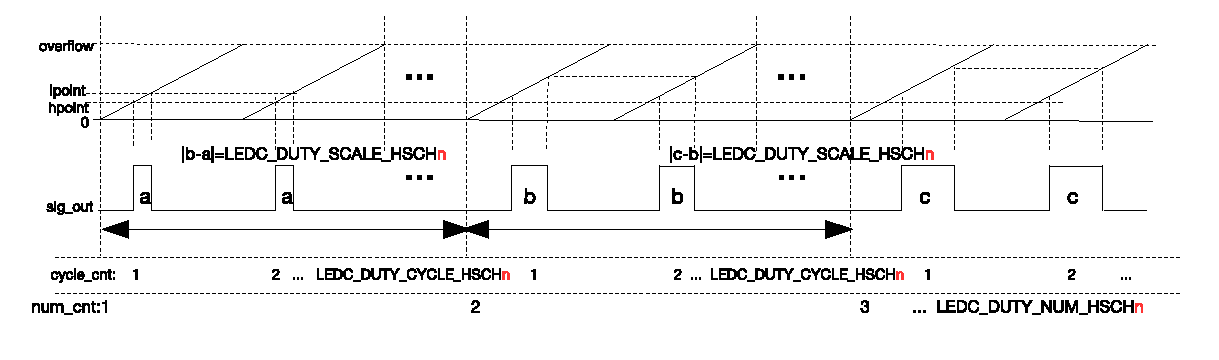
\includegraphics[width=0.7\textwidth]{./28-LEDPWM/figures/led_pwm_unfixed_duty}}
    \caption{渐变占空比输出信号图}
    \label{Figure:led_pwm_unfixed_duty}
\end{figure}

{\bfseries 注意}
\begin{itemize}
    \item 当 LEDC 处于渐变过程中，不支持操作（如暂停）渐变，或者配置以下寄存器：
    \begin{itemize}
    \item LEDC\_HPOINT\_H/LSCH\textcolor{red}{\it{n}}
    \item LEDC\_DUTY\_H/LSCH\textcolor{red}{\it{n}}
    \item LEDC\_DUTY\_START\_H/LSCH\textcolor{red}{\it{n}}
    \item LEDC\_DUTY\_INC\_H/LSCH\textcolor{red}{\it{n}}
    \item LEDC\_DUTY\_NUM\_H/LSCH\textcolor{red}{\it{n}}
    \item LEDC\_DUTY\_CYCLE\_H/LSCH\textcolor{red}{\it{n}}
    \item LEDC\_DUTY\_SCALE\_H/LSCH\textcolor{red}{\it{n}}
    \end{itemize}
    必须在 LEDC\_DUTY\_CHNG\_END\_HSCH\textcolor{red}{\it{n}} 或者 LEDC\_DUTY\_CHNG\_END\_LSCH\textcolor{red}{\it{n}} 中断之后才能进行第二次渐变配置。
    \item 当配置 LEDC 为递减渐变且 LEDC\_DUTY\_HSCH\textcolor{red}{\it{n}} 为 2$ ^{LEDC\_HSTIMER\textcolor{red}{\it{x}}\_DUTY\_RES}$ 时，不允许配置\\ LEDC\_DUTY\_SCALE\_HSCH\textcolor{red}{\it{n}} 为 1；当配置 LEDC 为递减渐变且 LEDC\_DUTY\_LSCH\textcolor{red}{\it{n}} 为 2$^ {LEDC\_LSTIMER\textcolor{red}{\it{x}}\_DUTY\_RES}$ 时，不允许配置 LEDC\_DUTY\_SCALE\_LSCH\textcolor{red}{\it{n}} 为 1。
\end{itemize}

\subsection{中断}
\begin{itemize}
\item \label{int:LEDCDUTYCHNGENDLSCHnINT}LEDC\_DUTY\_CHNG\_END\_LSCH\textcolor{red}{\it{n}}\_INT 低速通道上的占空比渐变结束触发中断。
\item \label{int:LEDCDUTYCHNGENDHSCHnINT}LEDC\_DUTY\_CHNG\_END\_HSCH\textcolor{red}{\it{n}}\_INT 高速通道上的占空比渐变结束触发中断。
\item \label{int:LEDCHSTIMERxOVFINT}LEDC\_HS\_TIMER\textcolor{red}{\it{n}}\_OVF\_INT 高速时钟计数器达到最大计数值触发中断。
\item \label{int:LEDCLSTIMERxOVFINT}LEDC\_LS\_TIMER\textcolor{red}{\it{n}}\_OVF\_INT 低速时钟计数器达到最大计数值触发中断。
\end{itemize}

\hypertarget{ledpwm-reg-summ}{}
\section{寄存器列表}\label{section:6.3}

本小节的所有地址均为相对于 SHA 加速器基地址的地址偏移量（相对地址），具体基地址请见章节 \ref{mod:sysmem} \textit{\nameref{mod:sysmem}} 中的表 \ref{table:Peripheral_Address_Mapping}。

请查看章节 \hyperref[glossary-access-types]{\textit{寄存器的访问类型}}，了解“访问”列缩写的含义。

\subfile{\modulefiles/ledc_reg_summary_cn.tex}
{\clearpage}

\section{寄存器}

本小节的所有地址均为相对于 LED PWM 基地址的地址偏移量（相对地址），具体基地址请见章节 \ref{mod:sysmem} \textit{\nameref{mod:sysmem}} 中的表 \ref{table:Peripheral_Address_Mapping}。寄存器绝对地址见章节 \ref{section:6.3} \textit{\nameref{section:6.3}}。

关于保留 (reserved) 域的处理，请查看章节 \hyperref[programming-reserved-field]{\textit{如何配置寄存器的保留域}}。

\subfile{\modulefiles/ledc_reg_cn.tex}

\end{document}
